\documentclass[aspectratio=169,10pt]{beamer}

% -------------------------------------------------
% Osnovne nastavitve
% -------------------------------------------------
\usepackage[utf8]{inputenc}
\usepackage[T1]{fontenc}
\usepackage[slovene]{babel}
\usepackage{lmodern}
\usepackage{amsmath,amssymb}
\usepackage{booktabs}
\usepackage{array}
\usepackage{graphicx}
\usepackage{tikz}
\graphicspath{{slike/}}

% -------------------------------------------------
% Barve (enake kot v prosojnicah v brskalniku)
% -------------------------------------------------
\definecolor{ink}{HTML}{14213D}
\definecolor{paper}{HTML}{FAF8F3}
\definecolor{body}{HTML}{4A5568}
\definecolor{muted}{HTML}{5B6B7F}
\definecolor{accent}{HTML}{2F6690}
\definecolor{hl}{HTML}{B5571A}
\definecolor{rule}{HTML}{D5DBE3}

\setbeamercolor{background canvas}{bg=paper}
\setbeamercolor{normal text}{fg=ink}
\setbeamercolor{frametitle}{fg=ink}
\setbeamercolor{itemize item}{fg=accent}
\setbeamertemplate{itemize item}[circle]
\setbeamertemplate{navigation symbols}{}
\setbeamerfont{frametitle}{series=\bfseries,size=\LARGE}

% Naslov prosojnice: nad njim kratka oznaka dela (podnaslov okvirja)
\setbeamertemplate{frametitle}{%
  \vspace*{5mm}%
  {\color{accent}\scriptsize\bfseries\MakeUppercase{\insertframesubtitle}}\par\vspace{1.2mm}%
  {\usebeamerfont{frametitle}\color{ink}\insertframetitle}\par\vspace{1mm}}

% Noga: vir na levi, številka prosojnice na desni
\makeatletter
\newcommand{\vir}[1]{\gdef\vir@besedilo{#1}}
\gdef\vir@besedilo{}
\setbeamertemplate{footline}{%
  \hspace*{8mm}\begin{minipage}[b]{0.82\paperwidth}\raggedright\color{muted}\tiny\vir@besedilo\end{minipage}%
  \hfill{\color{muted}\tiny\insertframenumber}\hspace*{8mm}\par\vspace*{4mm}}
\makeatother

% Kartica: modra črta zgoraj, krepki naslov, besedilo
\newcommand{\kartica}[2]{%
  {\color{accent}\rule{\linewidth}{1pt}}\par\vspace{1.5mm}%
  {\bfseries\normalsize #1}\par\vspace{1mm}%
  {\color{body}\small #2}}
\newcommand{\stevilka}[1]{{\color{accent}\bfseries\LARGE #1}}
\newcommand{\oznaka}[1]{{\color{accent}\scriptsize\bfseries\MakeUppercase{#1}}}

\title{Umetna inteligenca kot vir R\&R in dolgoročne gospodarske rasti}
\subtitle{ZDA v obdobju 2010--2025}
\author{Andraž Ajdovec \and Tin Cvek \and Jan Hrovat \and Miha Ručigaj}

\begin{document}

% =================================================
% 1 Naslovna (Andraž)
% =================================================
\begin{frame}[plain]
\vspace*{6mm}
{\color{hl}\rule{18mm}{1.2mm}}\par\vspace{3mm}
{\color{hl}\footnotesize\bfseries SEMINARSKA NALOGA · MAKROEKONOMIJA}\par\vspace{5mm}
\begin{minipage}{0.9\linewidth}\raggedright
{\color{ink}\fontsize{26}{30}\selectfont\bfseries Umetna inteligenca kot vir R\&R in dolgoročne gospodarske rasti}
\end{minipage}\par\vspace{5mm}
{\color{accent}\Large ZDA v obdobju 2010--2025}\par
\vfill
{\color{rule}\rule{\linewidth}{0.6pt}}\par\vspace{3mm}
{\color{ink}\normalsize Andraž Ajdovec · Tin Cvek · Jan Hrovat · Miha Ručigaj}\par\vspace{1mm}
{\color{muted}\footnotesize Mentor: Jan Grobovšek · Univerza v Ljubljani, Fakulteta za matematiko in fiziko}\par
\vspace*{4mm}
\note{ANDRAŽ: Lep pozdrav. Smo Andraž Ajdovec, Tin Cvek, Jan Hrovat in Miha Ručigaj. Predstavili bomo seminarsko nalogo Umetna inteligenca kot vir raziskav in razvoja ter dolgoročne gospodarske rasti: ZDA v obdobju od 2010 do 2025.}
\end{frame}

% =================================================
% 2 Motivacija in raziskovalno vprašanje (Andraž)
% =================================================
\begin{frame}{Zakaj rast in zakaj umetna inteligenca}{Uvod}
\vir{Viri: Polanec (2014, str. 4); Grobovšek (2026, pros. 59, 119--120 in 124); NSB (2025); Stanford HAI (2025)}
\begin{columns}[T,onlytextwidth]
\begin{column}{0.48\textwidth}
\stevilka{+49\,\%}\par
{\color{body}\small višji dohodek na prebivalca po 40 letih, če je letna rast višja za 1 o.\,t.}\par\vspace{4mm}
\stevilka{Tehnologija}\par
{\color{body}\small je po Solowovem modelu edini vir dolgoročne rasti BDP na delavca; ideje nastajajo z R\&R.}\par\vspace{4mm}
{\color{hl}\bfseries\LARGE ZDA: tehnološka meja}\par
{\color{body}\small največ vlagajo v R\&R in UI; ker že uporabljajo najboljše tehnologije, hitreje rastejo le z novimi idejami.}
\end{column}
\begin{column}{0.47\textwidth}
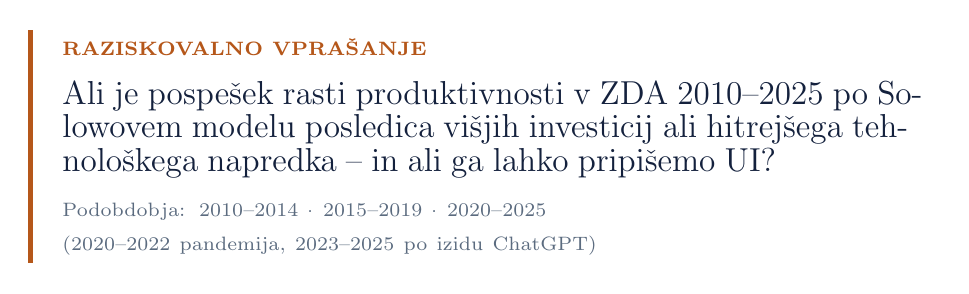
\begin{tikzpicture}
\node[text width=0.92\linewidth, inner sep=0pt, anchor=north west] (q) at (0,0) {%
  {\color{hl}\scriptsize\bfseries RAZISKOVALNO VPRAŠANJE}\par\vspace{2mm}
  {\color{ink}\large Ali je pospešek rasti produktivnosti v ZDA 2010--2025 po Solowovem modelu posledica višjih investicij ali hitrejšega tehnološkega napredka -- in ali ga lahko pripišemo UI?}\par\vspace{3mm}
  {\color{muted}\scriptsize Podobdobja: 2010--2014 · 2015--2019 · 2020--2025\\(2020--2022 pandemija, 2023--2025 po izidu ChatGPT)}};
\draw[hl, line width=2pt] ([xshift=-4mm,yshift=1mm]q.north west) -- ([xshift=-4mm,yshift=-1mm]q.south west);
\end{tikzpicture}
\end{column}
\end{columns}
\note{ANDRAŽ: Že majhne razlike v stopnji rasti so pomembne: če je letna rast višja za eno odstotno točko, je dohodek na prebivalca po 40 letih višji za približno 49 odstotkov. Po Solowovem modelu BDP na delavca dolgoročno raste le s tehnološkim napredkom, ta pa izvira iz idej, ki nastajajo z raziskavami in razvojem. Umetna inteligenca bi lahko bila nov vir idej, ocene njenega učinka pa se zelo razlikujejo. ZDA smo izbrali, ker največ vlagajo v raziskave in razvoj in v umetno inteligenco ter ker so na tehnološki meji. To pomeni, da že uporabljajo najboljše razpoložljive tehnologije, zato lahko hitreje rastejo le z novimi idejami, ne s posnemanjem drugih. Če UI pospešuje rast, bi se to moralo najprej pokazati prav v ZDA. Naše raziskovalno vprašanje je: ali je pospešek rasti produktivnosti v ZDA v obdobju od 2010 do 2025 po Solowovem modelu posledica višjih investicij ali hitrejšega tehnološkega napredka in ali ga lahko pripišemo umetni inteligenci? Obdobje smo razdelili na tri podobdobja, zadnje pa še na leta pandemije in leta po izidu ChatGPT.}
\end{frame}

% =================================================
% 3 Ključni podatki (Andraž)
% =================================================
\begin{frame}{Več R\&R in UI, investicije pri 18\,\% BDP}{Podatki}
\vir{Viri: NSB (2025); BEA (2026a, 2026b); NITRD (2021, 2024); Stanford HAI (2025); Pairolero in sod. (2025); BLS (2026b)}
\begin{columns}[c,onlytextwidth]
\begin{column}{0.44\textwidth}
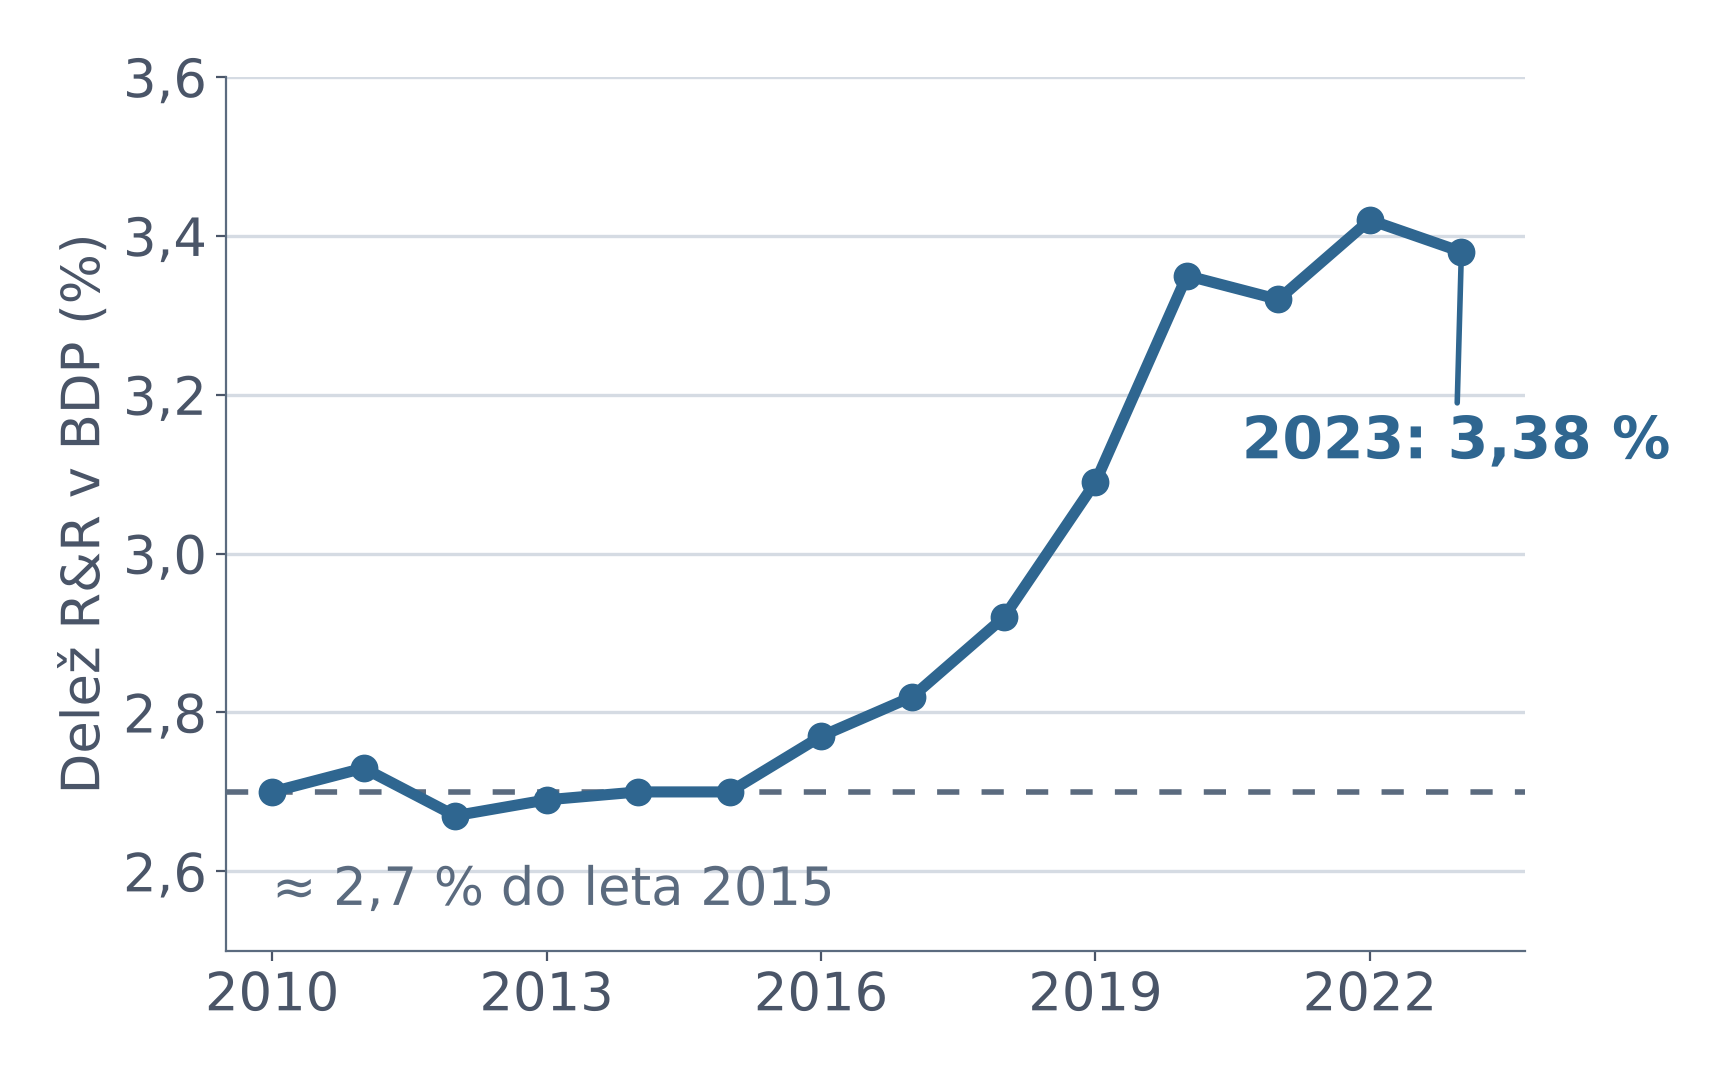
\includegraphics[width=\linewidth]{rnd.png}
\end{column}
\begin{column}{0.52\textwidth}
\renewcommand{\arraystretch}{1.1}
\begin{tabular}{@{}>{\raggedright\arraybackslash}p{0.27\linewidth}>{\raggedright\arraybackslash}p{0.70\linewidth}@{}}
{\color{accent}\bfseries\normalsize 3,38\,\%} & {\color{body}\scriptsize delež R\&R v BDP 2023 (do 2015 $\approx$\,2,7\,\%)}\\
{\color{accent}\bfseries\normalsize $\approx$\,18\,\%} & {\color{body}\scriptsize stopnja investicij $I/Y$ po letu 2015}\\
{\color{accent}\bfseries\normalsize 3,1 mrd \$} & {\color{body}\scriptsize vlaganja zvezne vlade v UI, FY2023 (FY2020: 1,4 mrd \$)}\\
{\color{accent}\bfseries\normalsize 109 mrd \$} & {\color{body}\scriptsize zasebne naložbe v UI v ZDA, 2024}\\
{\color{accent}\bfseries\normalsize +33\,\%} & {\color{body}\scriptsize UI-patentne prijave 2018--2023}\\
{\color{hl}\bfseries\normalsize 2,2\,\%} & {\color{body}\scriptsize rast BDP na uro 2020--25 (prej 1,1 in 1,4\,\%)}\\
\end{tabular}
\end{column}
\end{columns}
\note{ANDRAŽ: Podatke smo vzeli iz uradnih virov: izdatke za raziskave in razvoj od National Science Board, BDP in investicije od BEA, vlaganja v UI od programa NITRD in iz poročila AI Index, produktivnost pa od BLS. Izstopajo tri ugotovitve. Prvič, delež izdatkov za raziskave in razvoj v BDP je bil do leta 2015 okoli 2,7 odstotka, leta 2023 pa 3,38 odstotka. Drugič, celotna stopnja investicij se je ustalila pri okoli 18 odstotkih BDP. Tretjič, vlaganja v UI hitro rastejo: federalna (zvezna vlada ZDA) so se med letoma 2020 in 2023 več kot podvojila, zasebne naložbe pa so leta 2024 dosegle 109 milijard dolarjev. BDP na uro dela je v treh podobdobjih rasel po 1,1, 1,4 in 2,2 odstotka na leto. Ali je pospešek posledica investicij ali tehnologije, nam pove model, ki ga bo predstavil Tin.}
\end{frame}

% =================================================
% 4 Predpostavke in osnovni enačbi (Tin)
% =================================================
\begin{frame}{Predpostavke in osnovni enačbi}{Solowov model · 1/3}
\vir{Viri: Grobovšek (2026, pros. 15--21 in 52); Polanec (2014, str. 9--12)}
\begin{columns}[T,onlytextwidth]
\begin{column}{0.42\textwidth}
{\bfseries Predpostavke}\par\vspace{1mm}
\begin{itemize}\small\color{body}
\item Diskreten čas, reprezentativno podjetje in gospodinjstvo
\item Cobb--Douglas, konstantni donosi obsega
\item Popolna konkurenca: delež kapitala v dohodku $=\alpha$
\item Eksogena stopnja varčevanja $s$
\item Zaprto gospodarstvo: investicije $=$ varčevanje
\item Delo raste z $n$, tehnologija z $g$, amortizacija $\delta$
\end{itemize}
\end{column}
\begin{column}{0.52\textwidth}
\kartica{\oznaka{Proizvodnja}}{%
\[ Y_t=K_t^{\alpha}\,(A_tL_t)^{1-\alpha} \tag{1}\]
$A$ povečuje produktivnost dela, $\alpha$ je delež kapitala.}
\par\vspace{5mm}
\kartica{\oznaka{Kopičenje kapitala}}{%
\[ K_{t+1}=(1-\delta)\,K_t+s\,Y_t \tag{2}\]
Kapital po amortizaciji + investicije $s\cdot Y$.}
\end{column}
\end{columns}
\note{TIN: Uporabili smo Solowov model z rastjo prebivalstva in tehnologije v diskretnem času, kot je predstavljen na predavanjih. Gospodarstvo je zaprto, trgi so popolnoma konkurenčni, gospodinjstvo pa ničesar ne optimizira, temveč varčuje eksogen delež s dohodka. Delo raste po stopnji n, tehnologija po stopnji g, kapital pa se amortizira po stopnji delta. Proizvodnja je podana z enačbo ena. To je Cobb-Douglasova funkcija kapitala in učinkovitega dela, kjer A povečuje produktivnost dela, alfa pa je delež kapitala v dohodku. Ker so investicije enake varčevanju, se kapital kopiči po enačbi dve: kapital v naslednjem obdobju je kapital, ki ostane po amortizaciji, plus investicije, s krat Y.}
\end{frame}

% =================================================
% 5 Dinamika kapitala (Tin)
% =================================================
\begin{frame}{Dinamika kapitala na enoto učinkovitega dela}{Solowov model · 2/3}
\vir{Vir: Grobovšek (2026, pros. 16--21, 31 in 52--57)}
\[ \tilde k_t\equiv\frac{K_t}{A_tL_t},\qquad \tilde k_{t+1}=\frac{(1-\delta)\,\tilde k_t+s\,\tilde k_t^{\alpha}}{(1+g)(1+n)} \tag{3}\]
\begin{center}{\color{body}\small Dobimo jo, ko enačbo (2) delimo z $A\cdot L$ v naslednjem obdobju, tj. z $(1+g)(1+n)\cdot A\cdot L$.}\end{center}
\vspace{4mm}
\begin{columns}[T,onlytextwidth]
\begin{column}{0.31\textwidth}\kartica{Zakaj $K/(AL)$?}{$A$ in $L$ rasteta, zato kapital na delavca ne konvergira k stalni vrednosti.}\end{column}
\begin{column}{0.31\textwidth}\kartica{\color{accent}Pod ustaljeno vrednostjo}{$K$ in $Y$ rasteta hitreje kot učinkovito delo $AL$.}\end{column}
\begin{column}{0.31\textwidth}\kartica{\color{hl}Nad ustaljeno vrednostjo}{$K$ in $Y$ rasteta počasneje -- mejni produkt kapitala je padajoč.}\end{column}
\end{columns}
\note{TIN: Ker A in L rasteta, kapital na delavca ne konvergira k stalni vrednosti. Zato model zapišemo s kapitalom na enoto učinkovitega dela, k z valovnico, torej K deljeno z A krat L. Če enačbo dve delimo z A krat L v naslednjem obdobju, dobimo enačbo tri. Ko je k z valovnico pod ustaljeno vrednostjo, kapital raste hitreje kot učinkovito delo, ko je nad njo, pa počasneje. Razlog je padajoči mejni produkt kapitala.}
\end{frame}

% =================================================
% 6 Uravnotežena pot rasti (Tin)
% =================================================
\begin{frame}{Uravnotežena pot rasti}{Solowov model · 3/3}
\vir{Viri: Grobovšek (2026, pros. 40, 55--61 in 77); Polanec (2014, str. 9 in 18)}
\vspace{-2mm}
\[ \tilde k^{\star}=\left(\frac{s}{g+n+gn+\delta}\right)^{\frac{1}{1-\alpha}},\qquad y^{\star}_t=A_t\left(\frac{s}{g+n+gn+\delta}\right)^{\frac{\alpha}{1-\alpha}} \tag{4}\]
\[ \frac{K}{Y}=\frac{s}{g+n+gn+\delta}=\frac{0{,}2}{0{,}02+0{,}01+0{,}0002+0{,}06}\approx 2{,}2 \tag{5}\]
\begin{center}{\color{muted}\scriptsize Parametri: $\delta=0{,}06$ · $\alpha=0{,}33$ · $s=0{,}2$ (predavanja) · $g=2\,\%$ · $n=1\,\%$ (Polanec)}\end{center}
\vspace{2mm}
\begin{columns}[T,onlytextwidth]
\begin{column}{0.31\textwidth}\kartica{\color{accent}$y$ raste z $g$}{BDP na delavca je sorazmeren z $A$, zato dolgoročno raste s stopnjo $g$.}\end{column}
\begin{column}{0.31\textwidth}\kartica{\color{accent}$s$ določa raven}{Višje varčevanje zviša raven, ne pa dolgoročne rasti.}\end{column}
\begin{column}{0.31\textwidth}\kartica{\color{hl}$K/Y\approx 2{,}2$}{Konstanten, neodvisen od $A$ -- skladno s Kaldorjevim dejstvom.}\end{column}
\end{columns}
\note{TIN: Na uravnoteženi poti je k z valovnico konstanten. Če v enačbi tri izenačimo k v obeh obdobjih, dobimo enačbo štiri. Iz nje sledi ključno sporočilo modela: BDP na delavca je sorazmeren z A, zato dolgoročno raste s stopnjo g. Stopnja varčevanja vpliva le na raven, ne na rast. Iz istega pogoja sledi enačba pet: razmerje med kapitalom in BDP je na uravnoteženi poti konstantno in ni odvisno od A. S parametri s predavanj, delta 0,06, alfa 0,33 in s 0,2, ter z g 2 odstotka in n 1 odstotek je to razmerje okoli 2,2, kar se ujema s Kaldorjevim dejstvom. Kako model uporabimo na podatkih, bo predstavil Jan.}
\end{frame}

% =================================================
% 7 Računovodska razčlenitev (Jan)
% =================================================
\begin{frame}{Računovodska razčlenitev rasti}{Razčlenitev rasti}
\vir{Viri: Grobovšek (2026, pros. 64--81); Polanec (2014, str. 9 in 23); Garín in sod. (2021, str. 142)}
\[ y=A^{1-\alpha}k^{\alpha}h^{1-\alpha}\qquad\text{oziroma}\qquad y=A\left(\frac{K}{Y}\right)^{\frac{\alpha}{1-\alpha}}h \tag{6}\]
\[ g_y=g_A+\frac{\alpha}{1-\alpha}\,g_{K/Y}+g_h \tag{7}\]
\begin{center}{\color{body}\small $\alpha=\tfrac13\;\Rightarrow\;\dfrac{\alpha}{1-\alpha}=0{,}5$, \qquad $g_A\approx\dfrac{g_{\mathrm{TFP}}}{1-\alpha}$}\end{center}
\vspace{2mm}
\begin{columns}[T,onlytextwidth]
\begin{column}{0.31\textwidth}\kartica{Zakaj $K/Y$, ne $k$?}{$k$ je odvisen od $A$, $K/Y$ pa na uravnoteženi poti od $A$ ni odvisen.}\end{column}
\begin{column}{0.31\textwidth}\kartica{$A$ je ostanek}{Vse, česar ne pojasnita $K/Y$ in $h$; preverimo ga z uradno TFP.}\end{column}
\begin{column}{0.31\textwidth}\kartica{\color{hl}Preverljiva napoved}{Na uravnoteženi poti $K/Y$ ne raste, zato investicije ne prispevajo k rasti.}\end{column}
\end{columns}
\note{JAN: Za empirični del uporabimo računovodsko razčlenitev rasti s predavanj. Proizvodno funkcijo razširimo s človeškim kapitalom h in jo zapišemo na delavca. Dobimo prvi zapis v enačbi šest. Predavanje priporoča drugi zapis, v katerem namesto kapitala na delavca nastopa razmerje K proti Y. Kapital na delavca je namreč odvisen od A, saj boljša tehnologija poveča tudi investicije, razmerje K proti Y pa po enačbi pet od A ni odvisno. Če drugi zapis logaritmiramo in vzamemo časovno razliko, dobimo enačbo sedem: rast BDP na delavca je vsota rasti produktivnosti, prispevka razmerja K proti Y in rasti človeškega kapitala. Pri alfi ena tretjina je utež pri K proti Y enaka 0,5. Produktivnost A izmerimo kot ostanek in jo preverimo z uradno TFP, saj je TFP enaka A na ena minus alfa.}
\end{frame}

% =================================================
% 8 Štiri razlage in simulacija (Jan)
% =================================================
\begin{frame}{Štiri možne razlage pospeška}{Simulacija}
\vir{Vir: lastni izračun z enačbama (1) in (2); parametri Grobovšek (2026, pros. 40), Polanec (2014, str. 18); Jones (1995)}
\begin{columns}[c,onlytextwidth]
\begin{column}{0.49\textwidth}
\scriptsize
\renewcommand{\arraystretch}{1.3}
\begin{tabular}{@{}>{\raggedright\arraybackslash}p{0.27\linewidth}>{\raggedright\arraybackslash}p{0.18\linewidth}>{\raggedright\arraybackslash}p{0.30\linewidth}>{\raggedright\arraybackslash}p{0.15\linewidth}@{}}
\toprule
\textbf{Razlaga} & \textbf{Sprememba} & \textbf{Rast BDP na delavca} & \textbf{$K/Y$}\\
\midrule
(A) višje investicije & $s$: 0,20 $\to$ 0,21 & +0,15 o.\,t., nato nazaj na 2\,\% & naraste\\
(B) enkraten dvig $A$ & $A$ +3\,\% & eno obdobje 4,04\,\%, nato $\approx$\,2\,\% & pade, vrne se\\
(C) trajno višji $g$ & $g$: 2 $\to$ 2,5\,\% & takoj +0,33 o.\,t., nato $\to$ 2,5\,\% & rahlo pade\\
(D) več R\&R (Jones) & višji delež R\&R & nekaj let višja rast $A$ & kot (B)\\
\bottomrule
\end{tabular}
\par\vspace{4mm}
{\normalsize\bfseries Samo (C) trajno zviša rast. Le (A) poveča razmerje $K/Y$ -- to preverimo v podatkih.}
\end{column}
\begin{column}{0.48\textwidth}
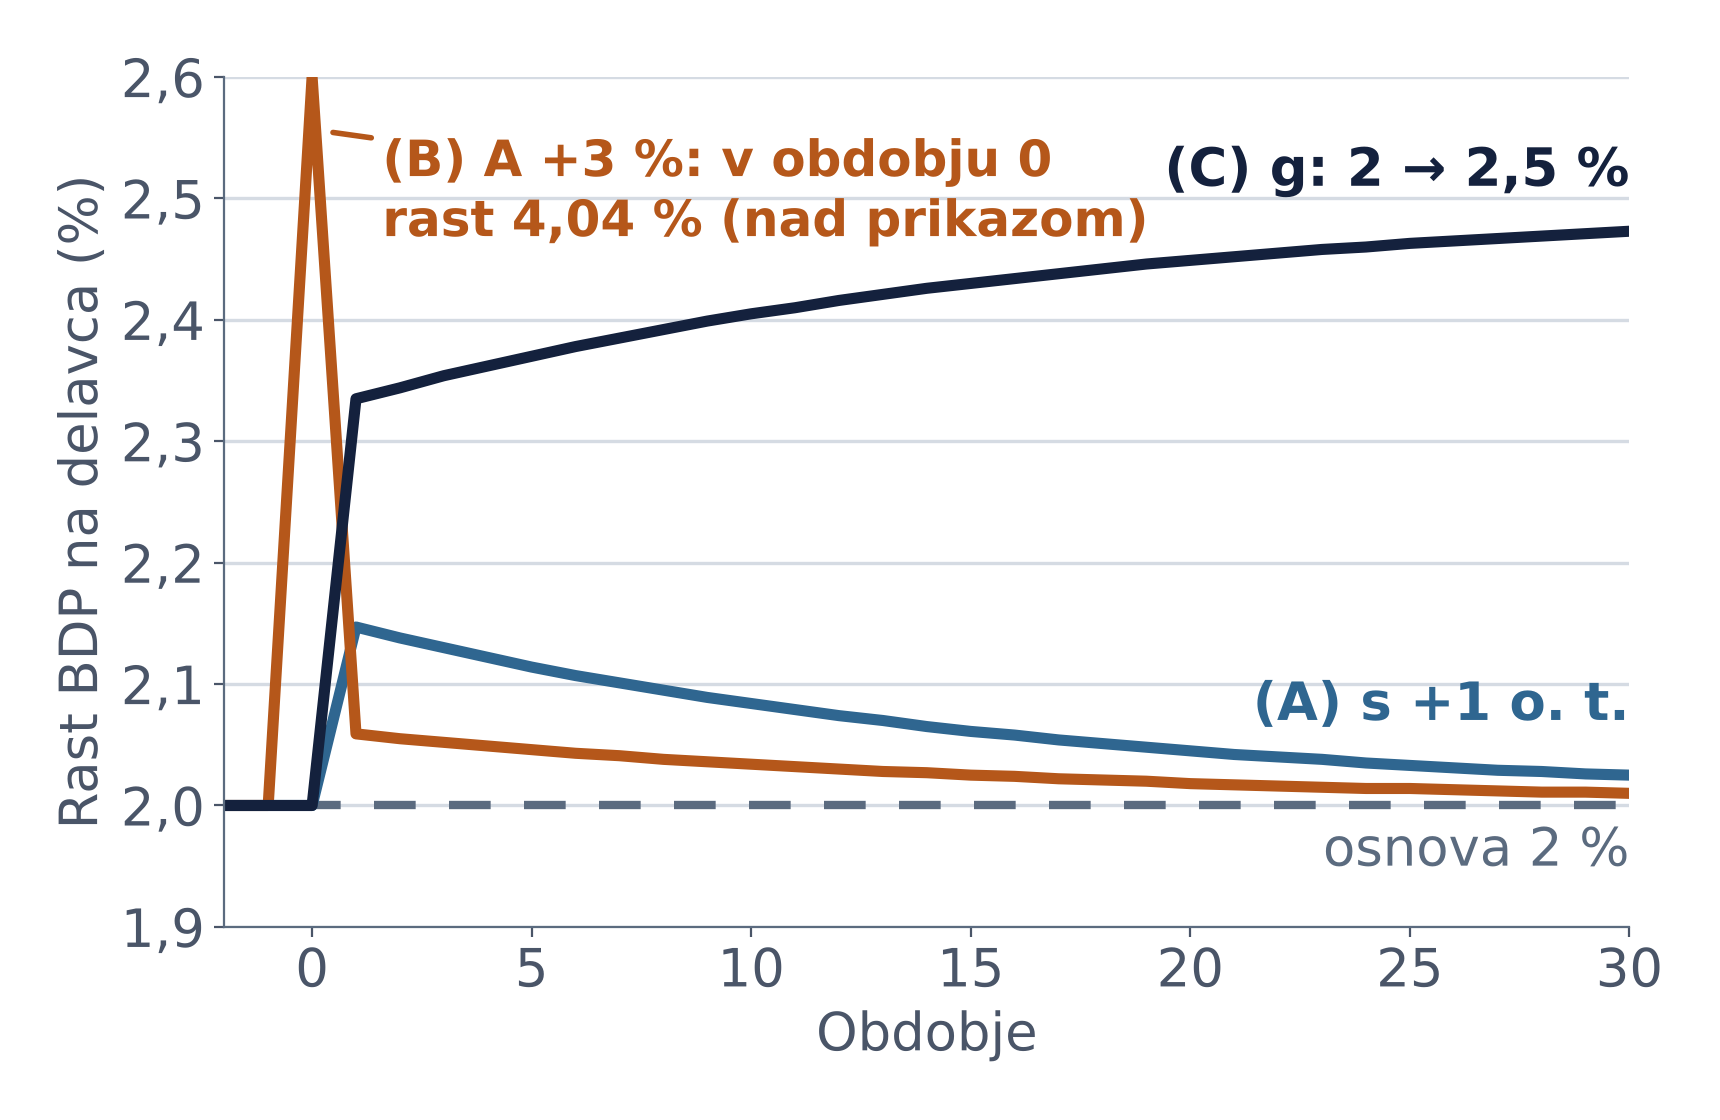
\includegraphics[width=\linewidth]{sim.png}
\end{column}
\end{columns}
\note{JAN: UI v modelu ne nastopa neposredno, zato jo vključimo kot spremembo parametrov modela. Tako dobimo štiri možne razlage pospeška, ki so v nalogi označene s črkami od A do D. Prve tri smo simulirali z enačbama ena in dve. Prva razlaga so višje investicije, na primer v podatkovne centre. Če se stopnja varčevanja poveča za eno odstotno točko, se rast v prvem letu poveča le za 0,15 odstotne točke, nato pa se vrne na 2 odstotka. Druga razlaga je enkraten dvig produktivnosti: če se A enkrat poveča za 3 odstotke, rast v tem letu skoči na 4 odstotke in se nato vrne na osnovo. Tretja razlaga je trajno hitrejši tehnološki napredek: če se g poveča z 2 na 2,5 odstotka, rast takoj naraste za 0,33 odstotne točke in se nato približuje 2,5 odstotka. Samo ta razlaga trajno zviša rast. Četrta razlaga izhaja iz Jonesovega modela: več raziskav in razvoja prinese nekaj let višjo rast produktivnosti, ne pa trajno. Ključno je, da razmerje K proti Y poveča le prva razlaga. Kaj kažejo podatki, bo predstavil Miha.}
\end{frame}

% =================================================
% 9 Razčlenitev po obdobjih (Miha)
% =================================================
\begin{frame}{Razčlenitev rasti BDP na uro dela po enačbi (7)}{Rezultati}
\vir{Viri: BLS (2026b); BEA (2026b); NSB (2025); lastni izračun. $\alpha=1/3$; * 2020--2023, ** 2023}
\footnotesize
\renewcommand{\arraystretch}{1.05}
\begin{tabular*}{\textwidth}{@{\extracolsep{\fill}}lrrrrr@{}}
\toprule
\textbf{Povprečna letna rast v \%} & \textbf{2010--14} & \textbf{2015--19} & \textbf{2020--25} & \textbf{2020--22} & {\color{hl}\textbf{2023--25}}\\
\midrule
\textbf{BDP na uro dela} & \textbf{1,10} & \textbf{1,44} & \textbf{2,23} & \textbf{1,96} & {\color{hl}\textbf{2,50}}\\
\quad produktivnost $A$ & 1,22 & 1,10 & 1,71 & 1,18 & {\color{hl}\textbf{2,25}}\\
\quad prispevek $K/Y$ ($0{,}5\cdot g_{K/Y}$) & $-0{,}48$ & $-0{,}06$ & $-0{,}05$ & 0,06 & {\color{hl}$-0{,}15$}\\
\quad človeški kapital $h$ & 0,36 & 0,40 & 0,56 & 0,72 & {\color{hl}0,40}\\
\midrule
Kontrola: $g_{\mathrm{TFP}}/(1-\alpha)$ po BLS & 1,22 & 1,02 & 1,55 & 1,11 & {\color{hl}1,99}\\
Investicije $I/Y$ (povprečje) & 16,0 & 17,8 & 18,1 & 18,0 & {\color{hl}18,1}\\
Delež R\&R v BDP (povprečje) & 2,70 & 2,86 & 3,37* & 3,36 & {\color{hl}3,38**}\\
\bottomrule
\end{tabular*}
\par\vspace{3mm}
\begin{columns}[T,onlytextwidth]
\begin{column}{0.31\textwidth}\kartica{2010--14}{$K/Y$ pada ($-0{,}48$) -- prilagajanje po recesiji.}\end{column}
\begin{column}{0.31\textwidth}\kartica{2015--19}{$I/Y$ +1,9 o.\,t., pospešek zaradi $K/Y$, ne $A$.}\end{column}
\begin{column}{0.31\textwidth}\kartica{\color{hl}2020--25}{Pospešek iz $A$, zgoščen v letih 2023--25.}\end{column}
\end{columns}
\note{MIHA: Hvala. V tabeli je razčlenitev rasti BDP na uro dela po enačbi sedem. Od 2010 do 2014 je razmerje K proti Y upadalo, kar je prilagajanje po recesiji. Od 2015 do 2019 se je stopnja investicij povečala in rast je pospešila na 1,44 odstotka, predvsem zaradi razmerja K proti Y. Od 2020 do 2025 je stopnja investicij ostala pri 18 odstotkih, rast BDP na uro pa je pospešila na 2,23 odstotka. Ta pospešek izvira iz produktivnosti, skoncentriran pa je v letih od 2023 do 2025, ko je produktivnost rasla po 2,25 odstotka.}
\end{frame}

% =================================================
% 10 Ujemanje z modelom (Miha)
% =================================================
\begin{frame}{Kako dobro je model napovedal?}{Rezultati}
\vir{Viri: tabela 4; simulacija (A); BEA (2026b); Polanec (2014, str. 18); lastni izračun}
\footnotesize
\renewcommand{\arraystretch}{1.2}
\begin{tabular}{@{}>{\raggedright\arraybackslash}p{0.29\textwidth}>{\raggedright\arraybackslash}p{0.40\textwidth}>{\raggedright\arraybackslash}p{0.25\textwidth}@{}}
\toprule
\textbf{Napoved modela} & \textbf{Podatki} & \textbf{Ujemanje}\\
\midrule
Na uravnoteženi poti je $K/Y$ konstanten & Prispevek $K/Y$: $-0{,}48\to-0{,}06\to-0{,}05$ & {\color{accent}\textbf{Da}} -- po letu 2015 se potrdi\\
Višje investicije zvišajo rast le malo (0,15 o.\,t. na o.\,t. višjega $s$) & 2015--19: napoved +0,28, dejansko +0,34 o.\,t.\newline 2020--25: napoved +0,03, dejansko +0,79 o.\,t. & {\color{hl}\textbf{Delno}} -- v 2015--19 da, v 2020--25 velik razkorak\\
Produktivnost raste s stalno stopnjo $g\approx2\,\%$ & Rast $A$: $1{,}22\to1{,}10\to1{,}71\,\%$\newline 2023--25: 2,25\,\% & {\color{hl}\textbf{Ne}} -- največje odstopanje\\
\bottomrule
\end{tabular}
\par\vspace{4mm}
{\normalsize Model dobro napove učinek investicij in razmerja $K/Y$, ne zna pa napovedati hitrosti tehnološkega napredka -- {\color{hl}$g$ je eksogen}, zato ves razkorak pripiše tehnologiji.}
\note{MIHA: Kako dobro je model napovedal? Preverimo lahko tri njegove napovedi. Prvič, da je razmerje K proti Y konstantno: to se po letu 2015 potrdi. Drugič, da višje investicije rast zvišajo le malo: za drugo obdobje model napove 0,28 odstotne točke pospeška, dejansko je bilo 0,34, kar se dobro ujema. Za tretje obdobje napove le 0,03, dejansko pa je bilo 0,79. Tretjič, da produktivnost dolgoročno raste s stalno stopnjo, za ZDA okoli 2 odstotka. Tu je odstopanje največje: do leta 2019 je rasla le po 1,1 do 1,2 odstotka, po letu 2023 pa po 2,25 odstotka. Model tega ne more napovedati, ker je g eksogen, zato ves razkorak pripiše tehnologiji.}
\end{frame}

% =================================================
% 11 Ali je to UI? (Miha)
% =================================================
\begin{frame}{Ali je pospešek posledica UI?}{Vloga umetne inteligence}
\vir{Viri: Acemoglu (2024, str. 29); Brynjolfsson in sod. (2018, str. 3); Jones (1995); NSB (2025); lastni izračun}
{\color{body}Rast produktivnosti $A$ je bila v letih 2023--2025 za \textbf{1,15 o.\,t.} višja kot v letih 2015--2019. Verjetno ne v celoti -- trije razlogi:}
\par\vspace{5mm}
\begin{columns}[T,onlytextwidth]
\begin{column}{0.31\textwidth}\kartica{\oznaka{1 · Velikost}\par\vspace{1mm}{\color{hl}\LARGE 0,1 o.\,t.}}{Ocena učinka UI (Acemoglu, 2024) v enotah $A$ -- manj kot desetina opaženega pospeška.}\end{column}
\begin{column}{0.31\textwidth}\kartica{\oznaka{2 · Časovni potek}\par\vspace{1mm}{\color{hl}\LARGE J-krivulja}}{Nove tehnologije izmerjeno produktivnost sprva podcenijo, zato takojšen skok po izidu ChatGPT ni prepričljiv.}\end{column}
\begin{column}{0.31\textwidth}\kartica{\oznaka{3 · Alternativa}\par\vspace{1mm}{\color{hl}\LARGE +0,67 o.\,t.}}{Delež R\&R v BDP se je po 2015 povečal; po Jonesu to z zamikom prehodno zviša rast $A$ -- brez UI.}\end{column}
\end{columns}
\note{MIHA: Ali je ta tehnološki napredek posledica UI? Menimo, da ne v celoti. Prvič, Acemoglujeva ocena učinka UI je manj kot desetina pospeška. Drugič, nove tehnologije izmerjeno produktivnost na začetku podcenijo, zato takojšen skok po izidu ChatGPT ni prepričljiv. Tretjič, pospešek enako dobro pojasni četrta razlaga, saj se je delež raziskav in razvoja po letu 2015 povečal.}
\end{frame}

% =================================================
% 12 Zaključek (Miha)
% =================================================
\begin{frame}[plain]
\vspace*{8mm}
{\color{hl}\footnotesize\bfseries ODGOVOR NA RAZISKOVALNO VPRAŠANJE}\par\vspace{6mm}
\begin{tabular}{@{}p{8mm}>{\raggedright\arraybackslash}p{0.85\textwidth}@{}}
{\color{hl}\fontsize{22}{26}\selectfont\bfseries 1} & {\fontsize{22}{26}\selectfont Pospešek je posledica hitrejšega tehnološkega napredka, ne višjih investicij.}\\[6mm]
{\color{hl}\fontsize{22}{26}\selectfont\bfseries 2} & {\fontsize{22}{26}\selectfont Jasnega učinka UI na produktivnost do leta 2025 še ne moremo zaznati.}\\
\end{tabular}
\vfill
{\color{rule}\rule{\linewidth}{0.6pt}}\par\vspace{3mm}
{\color{ink}\Large\bfseries Hvala za pozornost -- vprašanja?}\par
\vspace*{6mm}
\note{MIHA: Pospešek je torej posledica hitrejšega tehnološkega napredka, ne višjih investicij, jasnega učinka UI pa do leta 2025 še ne moremo zaznati. Hvala za pozornost, z veseljem odgovorimo na vprašanja.}
\end{frame}

\end{document}
